\documentclass[manuscript]{aastex6}

% to-do list
% ----------
% - Add references and uncertainties to Table 1

% style notes
% -----------
% - This file generates by Makefile; don't be typing ``pdflatex'' or some bullshit.
% - Line break between sentences to make the git diffs readable.
% - Use \, as a multiply operator.
% - Reserve () for function arguments; use [] or {} for outer shit.
% - Use \sectionname not Section, \figname not Figure, \documentname not Article or Paper or paper.

\include{gitstuff}
% ----------------------------------- %
% start of AASTeX mods by DWH and DFM %
% ----------------------------------- %

\setlength{\voffset}{0in}
\setlength{\hoffset}{0in}
\setlength{\textwidth}{6in}
\setlength{\textheight}{9in}
\setlength{\headheight}{0ex}
\setlength{\headsep}{\baselinestretch\baselineskip} % this is 2 lines in ``manuscript''
\setlength{\footnotesep}{0in}
\setlength{\topmargin}{-\headsep}
\setlength{\oddsidemargin}{0.25in}
\setlength{\evensidemargin}{0.25in}

\linespread{0.54} % close to 10/13 spacing in ``manuscript''
\setlength{\parindent}{0.54\baselineskip}
\hypersetup{colorlinks = false}
\makeatletter % you know you are living your life wrong when you need to do this
\long\def\frontmatter@title@above{
\vspace*{-\headsep}\vspace*{\headheight}
\noindent\footnotesize
{\noindent\footnotesize\textsc{\@journalinfo}}\par
{\noindent\scriptsize Preprint typeset using \LaTeX\ style AASTeX6
with modifications by DWH and DFM.
}\par\vspace*{-\baselineskip}\vspace*{0.625in}
}%
\long\def\frontmatter@abstractheading{%
\makeaffils
  \vspace*{-\baselineskip}\vspace*{1.5pt}
  \vspace*{0.13189in}
 \begingroup
  \centering
  \abstractname
  \vskip 1mm
  \par
 \endgroup
 \everypar{\rightskip=0.0in\leftskip=\rightskip}\par
}%
\def\frontmatter@keys@format{\vspace*{0.5mm}%
  \settowidth{\keys@width}{\normalsize\@keys@name}%
  \rightskip=0.0in\leftskip=\rightskip\parindent=0pt%
    \hangindent=\keys@width\hangafter=1\normalsize\raggedright}%
\def\twodigits#1{\ifnum#1<10 0\fi\the#1}
\def\mydate{\leavevmode\hbox{\the\year-\twodigits\month-\twodigits\day}}
\makeatother
\renewcommand{\today}{\mydate}

% Section spacing:
\makeatletter
\let\origsection\section
\renewcommand\section{\@ifstar{\starsection}{\nostarsection}}
\newcommand\nostarsection[1]{\sectionprelude\origsection{#1}}
\newcommand\starsection[1]{\sectionprelude\origsection*{#1}}
\newcommand\sectionprelude{\vspace{1em}}
\let\origsubsection\subsection
\renewcommand\subsection{\@ifstar{\starsubsection}{\nostarsubsection}}
\newcommand\nostarsubsection[1]{\subsectionprelude\origsubsection{#1}}
\newcommand\starsubsection[1]{\subsectionprelude\origsubsection*{#1}}
\newcommand\subsectionprelude{\vspace{1em}}
\makeatother

\widowpenalty=10000
\clubpenalty=10000

\sloppy\sloppypar

% ------------------ %
% end of AASTeX mods %
% ------------------ %


% packages
\definecolor{cbblue}{HTML}{3182bd}
\usepackage{microtype}  % ALWAYS!
\usepackage{amsmath,amssymb,natbib}
\usepackage[flushleft]{threeparttable}
\hypersetup{backref,breaklinks,colorlinks,urlcolor=cbblue,linkcolor=cbblue,citecolor=black}
\graphicspath{{figures/}}
\bibliographystyle{aasjournal.bst}

% define macros for text
\newcommand{\project}[1]{\textsl{#1}}
\newcommand{\acronym}[1]{{\small{#1}}}
\newcommand{\gaia}{\project{Gaia}}
\newcommand{\rave}{\project{\acronym{RAVE}}}
\newcommand{\apogee}{\project{\acronym{APOGEE}}}
\newcommand{\tmass}{\project{\acronym{2MASS}}}
\newcommand{\documentname}{Article}
\newcommand{\sectionname}{Section}
\newcommand{\figname}{Figure}
\newcommand{\eqname}{Equation}
\newcommand{\dr}{\acronym{DR1}}
\newcommand{\tgas}{\acronym{TGAS}}
\newcommand{\etal}{\textit{et al}.}
\newcommand*\elem[1]{\ensuremath{\mathrm{#1}}}
\newcommand*\elemH[1]{\ensuremath{[\mathrm{#1}/\elem{H}]}}
\newcommand*\teff{\ensuremath{T_\mathrm{eff}}}
\newcommand*\logg{\ensuremath{\log{g}}}
\newcommand*{\feh}{\ensuremath{\elemH{Fe}}}
\newcommand{\sunanalog}{\text{Krios}}
\newcommand{\bizarreone}{\text{Kronos}}
\newcommand{\Tcondens}{\ensuremath{T_C}}
\newcommand{\mearth}{\ensuremath{M_\oplus}}
\newcommand{\mjupiter}{\ensuremath{M_\mathrm{Jup}}}


% define macros for math
\newcommand{\given}{\,|\,}
\newcommand{\normal}{{\mathcal{N}}}
\newcommand{\dd}{\mathrm{d}}
\newcommand{\transp}[1]{{#1}^{\!\mathsf{T}}}
\newcommand{\inv}[1]{{#1}^{-1}}
\newcommand{\bs}[1]{\boldsymbol{#1}}
\newcommand{\vperp}{\bs{v}^\perp}
\newcommand{\propm}{\bs{\mu}}
\newcommand{\mat}[1]{\mathbf{#1}}
\renewcommand{\vec}[1]{\bs{#1}}
\newcommand{\kms}{\ensuremath{\rm km~s^{-1}}}
\newcommand{\msun}{{\rm M}_\odot}
\newcommand{\pc}{{\rm pc}}
\newcommand{\data}{\mathrm{data}}
\newcommand{\snr}{[S/N]_\varpi}
\newcommand{\eye}{\mathbb{I}}
\newcommand{\absdvtan}{\ensuremath{|\Delta\vec v_\mathrm{t}|}}
\newcommand{\estimates}{\ensuremath{\{\hat{\varpi_i},\hat{\mu_{\alpha,i}},\hat{\mu_{\delta,i}},\hat{v_{r,i}}\}}}

\newcommand{\todo}[1]{{\color{blue}TODO:#1}}

\renewcommand\tablename{Table}

\begin{document}\sloppy\sloppypar\raggedbottom\frenchspacing % trust me

\title{Kronos \& Krios: TBD}

\author{
  Semyeong Oh\altaffilmark{\pu,\lead},
  APW, JMB, KH, NL, DWH, DNS \etal\
}

% Affiliations
\newcommand{\pu}{1}
\newcommand{\lead}{2}
\newcommand{\ccpp}{3}
\newcommand{\mpia}{4}
\newcommand{\cca}{5}

\altaffiltext{\pu}{Department of Astrophysical Sciences,
                   Princeton University, Princeton, NJ 08544, USA}
\altaffiltext{\lead}{To whom correspondence should be addressed:
                     \texttt{semyeong@astro.princeton.edu}}
\altaffiltext{\ccpp}{Center for Cosmology and Particle Physics,
                     Department of Physics,
                     New York University, 4 Washington Place,
                     New York, NY 10003, USA}
\altaffiltext{\mpia}{Max-Planck-Institut f\"ur Astronomie,
                     K\"onigstuhl 17, D-69117 Heidelberg, Germany}
\altaffiltext{\cca}{Center for Computational Astrophysics, 162 5th Ave, New York, NY 10003, USA}


\begin{abstract}
  We report and discuss the discovery of a comoving pair of bright solar-type
  stars, HD~240430 and HD~240429, with a significant difference in their chemical
  abundance patterns.
  The two stars are co-spatial ($|\Delta \bs{x}| < XX~\pc$) at a distance of
  $r\approx 100~\pc$ with nearly identical three-dimensional velocities
  ($|\Delta \bs{v}| < XX~\kms$ with 95\% confidence), as inferred from \gaia\
  \tgas\ proper motions and high resolution radial velocity measurements.
  Both stars are young with ages $\approx$$500~{\rm Myr}$ as estimated from
  their lithium abundances, favoring the idea that they were born together and
  are or were recently a bound, wide binary system.
  However, the metallicities and chemical abundances of refractory
  elements in the two stars are very different, challenging this simple picture.
  In order to reconcile the seemingly contradictory observations,
  we consider scenarios in which the pair is unrelated despite
  its current spatial and kinematic configuration, and
  those in which the pair formed together but may now have different chemistry.
  In the latter, we consider the possibility that the more metal-rich of the two,
  \bizarreone, accreted $\approx$10's of Earth masses of protoplanetary, rocky material,
  selectively enhancing the refractory elements.
  Direct-imaging and precision radial velocity follow-up to study the existence
  or properties of planetary systems around these stars would help distinguish
  these scenarios.
\end{abstract}

\section{Introduction} % (fold)
\label{sec:introduction}

Wide binaries are valuable tools for studying star and planet formation as well
as Galactic dynamics and chemical evolution.
In the context of studying the evolution of the Milky Way, they are useful for
two main reasons.
First, because wide binaries are weakly bound systems that may be tidally
disrupted by e.g., field stars, molecular clouds, or the Galactic tidal field,
their statistics can be informative of the Galactic mass distribution.
For example, the separation distribution of halo binaries has been
used to constrain the mass of massive compact halo objects (\citealt{Yoo:2004aa}).
On the other hand, they are also prime targets to test the chemical tagging
hypothesis that stars of the same birthplace may be traced back by detailed
chemical abundance patterns as birth ``tag''s (\citealt{2002ARA&A..40..487F}).
A multiple-star system of any size that we believe are born together can serve this purpose,
with massive open clusters at one extreme.
Wide binaries are at the other extreme in that we may be less confident of
the coevality of individual systems
but they are much more abundant than the larger systems like open clusters,
rendering their statistics a meaningful indication of whether the hypothesis works.

Independently, in efforts to connect the host star's chemistry to
its planetary system, wide binaries with similar or very different planetary architectures around
the component stars are particularly useful as chemical signatures related to planet formation or accretion
can be revealed in a differential sense without any regard to the Galactic chemical evolution
as long as we assume that the two stars should have been born together with identical composition.
For close-in giant planets, it has been established that the planet-metallicity relation
is primordial, and that the enhanced metallicity in giant planet-hosting stars likely
promoted the formation of giant planets (\citealt{Fischer:2005aa}) by increasing
the availability of small particle condensates that forms planetesimals.
On the other hand, if host stars are to be polluted after their birth
by rocky planetary material with high refractory-to-volatile ratio,
the convective envelope of the stars may be enhanced in refractory elements (e.g., \elem{Fe})
compared to their initial state.
Thus, differing planet formation or accretion in the two otherwise identical stars
may imprint a difference of chemical abundances that depends on the
condensation temperature (\Tcondens).
Several systems in which at least one star hosts at least one planet
have been studied so far with high resolution spectroscopy in this context
(\citealt{Teske:2013aa,Mack:2014aa,Liu:2014aa,Teske:2015aa,Saffe:2015aa,
  Ramirez:2015aa,Biazzo:2015aa,Mack:2016aa,Teske:2016aa,Teske:2016ab}).
The results and interpretations of these studies are varied:
while some systems (e.g., HAT-P-1 (\citealt{Liu:2014aa}),
HD~20782/1 (\citealt{Mack:2014aa}), HD~80606/7 (\citealt{Saffe:2015aa,Mack:2014aa});
see also \citealt{Desidera:2004aa,Gratton:2001aa})
found no difference, other studies (e.g., XO-2 (\citealt{Teske:2015aa,Ramirez:2015aa,Biazzo:2015aa}))
have found a \Tcondens-dependent difference in abundance.
The increasing difference of abundance with condensation temperature
has been attributed both to more yet-undiscovered rocky planets around
the relatively refractory-poor star and to late time accretion of
refractory-rich planetary material (\citealt{Ramirez:2015aa,Biazzo:2015aa}.
% maybe want to point out the former interpretation roots back to melendez+09
% and some doubt to that interpretation...

So far the strongest evidence for accretion of planetary material by a host star comes
from spectral analysis of polluted white dwarfs (WDs).
Because the gravitational settling times of elements heavier than \elem{He} in
atmosphere is much shorter than the WD cooling time essentially providing a
clean slate for any sign of accretion, detection of metals indicates a
reservoir of dusty material around the WD.
Indeed, many of the polluted WDs have been shown to own a dusty disk detected
in the infrared.
Some of the most dramatically polluted WDs were revealed to have
surface abundances closely matched by rocky planetary material
indicated by e.g., bulk Earth composition, strongly arguing
that the disk formed from tidally disrupted minor planets
(\citealt{Zuckerman:2007aa,Klein:2010aa}).
Recently, transit signals from small bodies orbiting around a polluted WD
has been detected by \project{Kepler} adding further support to the picture
(\citealt{2015Natur.526..546V}).

Here, we report and discuss the discovery of a comoving pair of solar twin stars,
HD~240430 and HD~240429, with unusual chemical abundance and differential abundance patterns
that strongly suggest a dramatic accretion of planetary material by the two stars.
We nickname the two stars \bizarreone\ (HD~240430) and
\sunanalog\ (HD~240429) throughout the \documentname.
In \sectionname~\ref{sec:data} we present the astrometric and spectroscopic data
about the two stars relevant to the present discussion.
In \sectionname~\ref{sec:discussion} we discuss possible interpretations of
the abundance difference between the pair.
We summarize or discussions in \sectionname~\ref{sec:summary}.


\section{Data}
\label{sec:data}

\begin{deluxetable*}{c|cccc}
  \tablecaption{Astrometric and spectroscopic measurements of the pair
  \label{tab:kk}}
\tablehead{
  \colhead{}     & \colhead{}      & \sunanalog\         & \bizarreone\        & \colhead{} \\
  \colhead{Name} & \colhead{Units} & \colhead{HD 240429} & \colhead{HD 240430} & \colhead{Uncertainties}
}
\startdata
Sp Type                             &                & G0                     & G2                     &       \\
R.A.\tablenotemark{a}               & hh:mm:ss       & 23:51:55.21            & 23:52:09.42            &       \\
Dec.\tablenotemark{a}               & dd:mm:ss       & 59:42:48.16            &  59:42:26.08           &       \\
2MASS $J$\tablenotemark{a}          & mag            & $8.593 \pm 0.023$      & $8.415 \pm 0.026$      &       \\
$T_\mathrm{eff}$                    & K              & 5878                   & 5803                   & 25    \\
$\log{g}$                           &                & 4.43                   & 4.33                   & 0.028 \\
$v\sin{i}$                          & \kms\          & 1.1                    & 2.5                    &       \\
$[\elem{Fe}/\elem{H}]$              &                & 0.01                   & 0.20                   & 0.010 \\
Age\tablenotemark{b}                & Gyr            & $4.00_{-1.56}^{+1.51}$ & $4.28_{-1.03}^{+1.11}$ &       \\
$v_r$                               & \kms\          & $-21.2$                & $-21.2$                & 0.2   \\
$\varpi$\tablenotemark{a}          & mas            & $9.35 \pm 0.24$        & $9.41 \pm 0.25$        &       \\
$\mu_\alpha^*$\tablenotemark{a}    & mas\,yr$^{-1}$ & $89.25 \pm 0.66$       & $89.41 \pm 0.69$       &       \\
$\mu_\delta$\tablenotemark{a}      & mas\,yr$^{-1}$ & $-29.68 \pm 0.54$      & $-30.12 \pm 0.52$      &       \\
\hline
\multicolumn{5}{c}{$T_c < 1200$~K} \\
\hline
$A(\elem{Li})$\tablenotemark{c}    &                & $2.25$                 & $2.75$                 &       \\
$\elemH{C}$                         &                & $0.00$                 & $0.09$                 & 0.026 \\
$\elemH{N}$                         &                & $-0.06$                & $-0.01$                & 0.042 \\
$\elemH{O}$                         &                & $0.01$                 & $0.09$                 & 0.036 \\
$\elemH{Na}$                        &                & $-0.06$                & $-0.04$                & 0.014 \\
$\elemH{Mn}$                        &                & $-0.03$                & $0.00$                 & 0.020 \\
\hline
\multicolumn{5}{c}{$T_c > 1200$~K} \\
\hline
$\elemH{Mg}$                        &                & $0.01$                 & $0.19$                 & 0.012 \\
$\elemH{Al}$                        &                & $0.01$                 & $0.21$                 & 0.028 \\
$\elemH{Si}$                        &                & $0.00$                 & $0.16$                 & 0.008 \\
$\elemH{Ca}$                        &                & $0.02$                 & $0.23$                 & 0.014 \\
$\elemH{Ti}$                        &                & $0.02$                 & $0.20$                 & 0.012 \\
$\elemH{V}$                         &                & $0.02$                 & $0.20$                 & 0.034 \\
$\elemH{Cr}$                        &                & $0.01$                 & $0.17$                 & 0.014 \\
$\elemH{Fe}$                        &                & $0.01$                 & $0.20$                 & 0.010 \\
$\elemH{Ni}$                        &                & $-0.01$                & $0.21$                 & 0.014 \\
$\elemH{Y}$                         &                & $0.04$                 & $0.26$                 & 0.030 \\
\enddata
\tablenotetext{a}{From \tgas.}
\tablenotetext{b}{Derived in this work by isochrone fitting
  using the Yale-Yonsei model isochrones (\citealt{2013ApJ...776...87S}).}
\tablenotetext{c}{Absolute abundances from \citealt{jmlithium}.}
\tablecomments{
  All values are from \citealt{2016ApJS..225...32B} unless otherwise noted.
  The microturbulence parameter is fixed at $0.85$~\kms\ (\citealt{2015ApJ...805..126B}).
}
\end{deluxetable*}


Though previously recognized as a visual double star system
(\citealt{2001AJ....122.3466M}), \sunanalog\ and \bizarreone\ were identified as a
candidate comoving star pair in our recent search for comoving stars using the
proper motions and parallaxes from the \tgas catalog, a component of \gaia\ \dr\
(the astrometric measurements are listed in \tablename~\ref{tab:kk}).
We refer the readers to this previous work (\citealt{2016arXiv161202440O}) for a
full explanation of the methodology behind this search and only briefly describe
the method here.
For a given pair, we compute a marginalized likelihood ratio between the
hypotheses (1) that a given pair of stars share the same 3D velocity vector, and
(2) that they have independent 3D velocity vectors, both given only observations
of two components of the velocities (proper motions).
We then select a sample of high-confidence comoving star pairs by making a
conservative cut on this likelihood ratio.
In the resulting catalog of comoving pairs (\citealt{2016arXiv161202440O}),
the pair presented in this paper was assigned a group id of 1199,
and the marginalized likelihood ratio (Bayes factor)
between the two hypotheses is $\ln{\mathcal{L}_1/\mathcal{L}_2} = 8.52$,
well above the adopted cut value of 6.
We have checked that we do not find any possible additional comoving companions
by lowering the likelihood ratio cut for the stars around this pair.

In a separate effort to study detailed chemical abundances of
potential planet-hosting stars, \citet{2016ApJS..225...32B}
analyzed high resolution spectra of both stars obtained using HIRES spectrograph
on Keck~I telescope.
The spectral resolution is \todo{$R\approx XXX$} and the wavelength coverage is \todo{$XXX-XXX$~\AA}.
The resulting measurements include abundances measured for 15
chemical species (C, N, O, Na, Mg, Al, Si, Ca, Ti, V, Cr, Mn, Fe, Ni, Y) as
well as high precision radial velocities.
Other stellar parameters derived from these spectra are included in
\tablename~\ref{tab:kk}.

Combining these precise radial velocities with the \gaia\ astrometry, we can
compare differences between the inferred 6D phase-space properties for the
two stars.
We start by generating posterior samples over the Heliocentric distance, $r$,
tangential velocities, $(v_\alpha, v_\delta)$, and radial velocity, $\hat{v}_r$,
given the observed parallax, $\pi$, and proper motion components,
$(\mu_{\alpha^*}, \mu_\delta)$, and radial velocity, $v_r$.
By defining the vectors
% SMOH: I understand you meant hat v_r as the latent true radial velocity but
% personally think a) it can confuse some people that there are hat quantities
% with no-hat quantities for hat-y vector and thus b) it'd be better to use hat
% quantities for observed variables and no-hat for latent true ones.
% SMOH: v_r is missing in the LHS of eq(3)
\begin{eqnarray}
  \vec{y} &=&
      \transp{\left(
        \begin{array}{c@{\hspace{1em}} c@{\hspace{1em}} c@{\hspace{1em}} c}
          \pi &
          \mu_{\alpha^*} &
          \mu_\delta &
          v_r
        \end{array}
      \right)}\\
  \hat{\vec{y}} &=&
      \transp{\left(
        \begin{array}{c@{\hspace{1em}} c@{\hspace{1em}} c@{\hspace{1em}} c}
          r^{-1} &
          r^{-1}\,v_\alpha &
          r^{-1}\,v_\delta &
          \hat{v}_r
        \end{array}
      \right)}
\end{eqnarray}
and by considering the covariance matrix $\mat{C}$ between the observed
quantities (provided by \tgas\ and extended to include the uncorrelated radial
velocity uncertainty), the likelihood can be written
\begin{eqnarray}
p(\pi, \mu_{\alpha^*}, \mu_\delta \given r, v_\alpha, v_\delta) &=&
  \left[\det\left(\frac{\mat{C}^{-1}}{2\pi}\right)\right]^{1/2} \,
    \exp \left[ -\frac{1}{2} \transp{\left(\vec{y} - \hat{\vec{y}} \right)} \,
    \mat{C}^{-1} \,
    \left(\vec{y} - \hat{\vec{y}} \right) \right] \label{eq:likefn} \quad .
\end{eqnarray}
We adopt a uniform space density prior for the distance and an isotropic
Gaussian for any velocity component, $v$, with a dispersion $\sigma_v=25~\kms$
\begin{eqnarray}
p(r) &=&
  \begin{cases}
    \frac{3}{r_{\rm lim}^3} \, r^2 & \text{if } 0 < r < r_{\rm lim}\\
    0              & \text{otherwise}
  \end{cases}\\
p(v) &=& \frac{1}{\sqrt{2\pi}\,\sigma_v} \,
  \exp\left[-\frac{1}{2} \, \frac{v^2}{\sigma_v^2} \right] \quad .
\end{eqnarray}
For each of the two stars, we use \project{emcee}
(\citealt{Foreman-Mackey:2013}) to generate posterior samples in $(r, v_\alpha,
v_\delta, \hat{v}_r)$ by running 64 walkers for 4608 steps and discarding the
first 512 steps as the burn-in period.
For each sample, we convert the heliocentric phase-space coordinates into
Galactocentric coordinates assuming the Sun's position and velocity are $x_\odot
= (-8.3, 0, 0)~{\rm kpc}$ and $v_\odot = (10, 244, 7.17)~\kms$ (\citealt{bovy,
etc.}).
\figname~\ref{fig:dxdv} shows differences in posterior samples converted to
Galactocentric phase-space coordinates for the two stars.
In all components, the pair is consistent with being comoving and close in
separation; the sky-projected separation of the two stars is $\approx$$0.01~\pc$
but the median 3-space separation is $\approx$$0.6~\pc$.

\begin{figure}[htbp]
  \begin{center}
    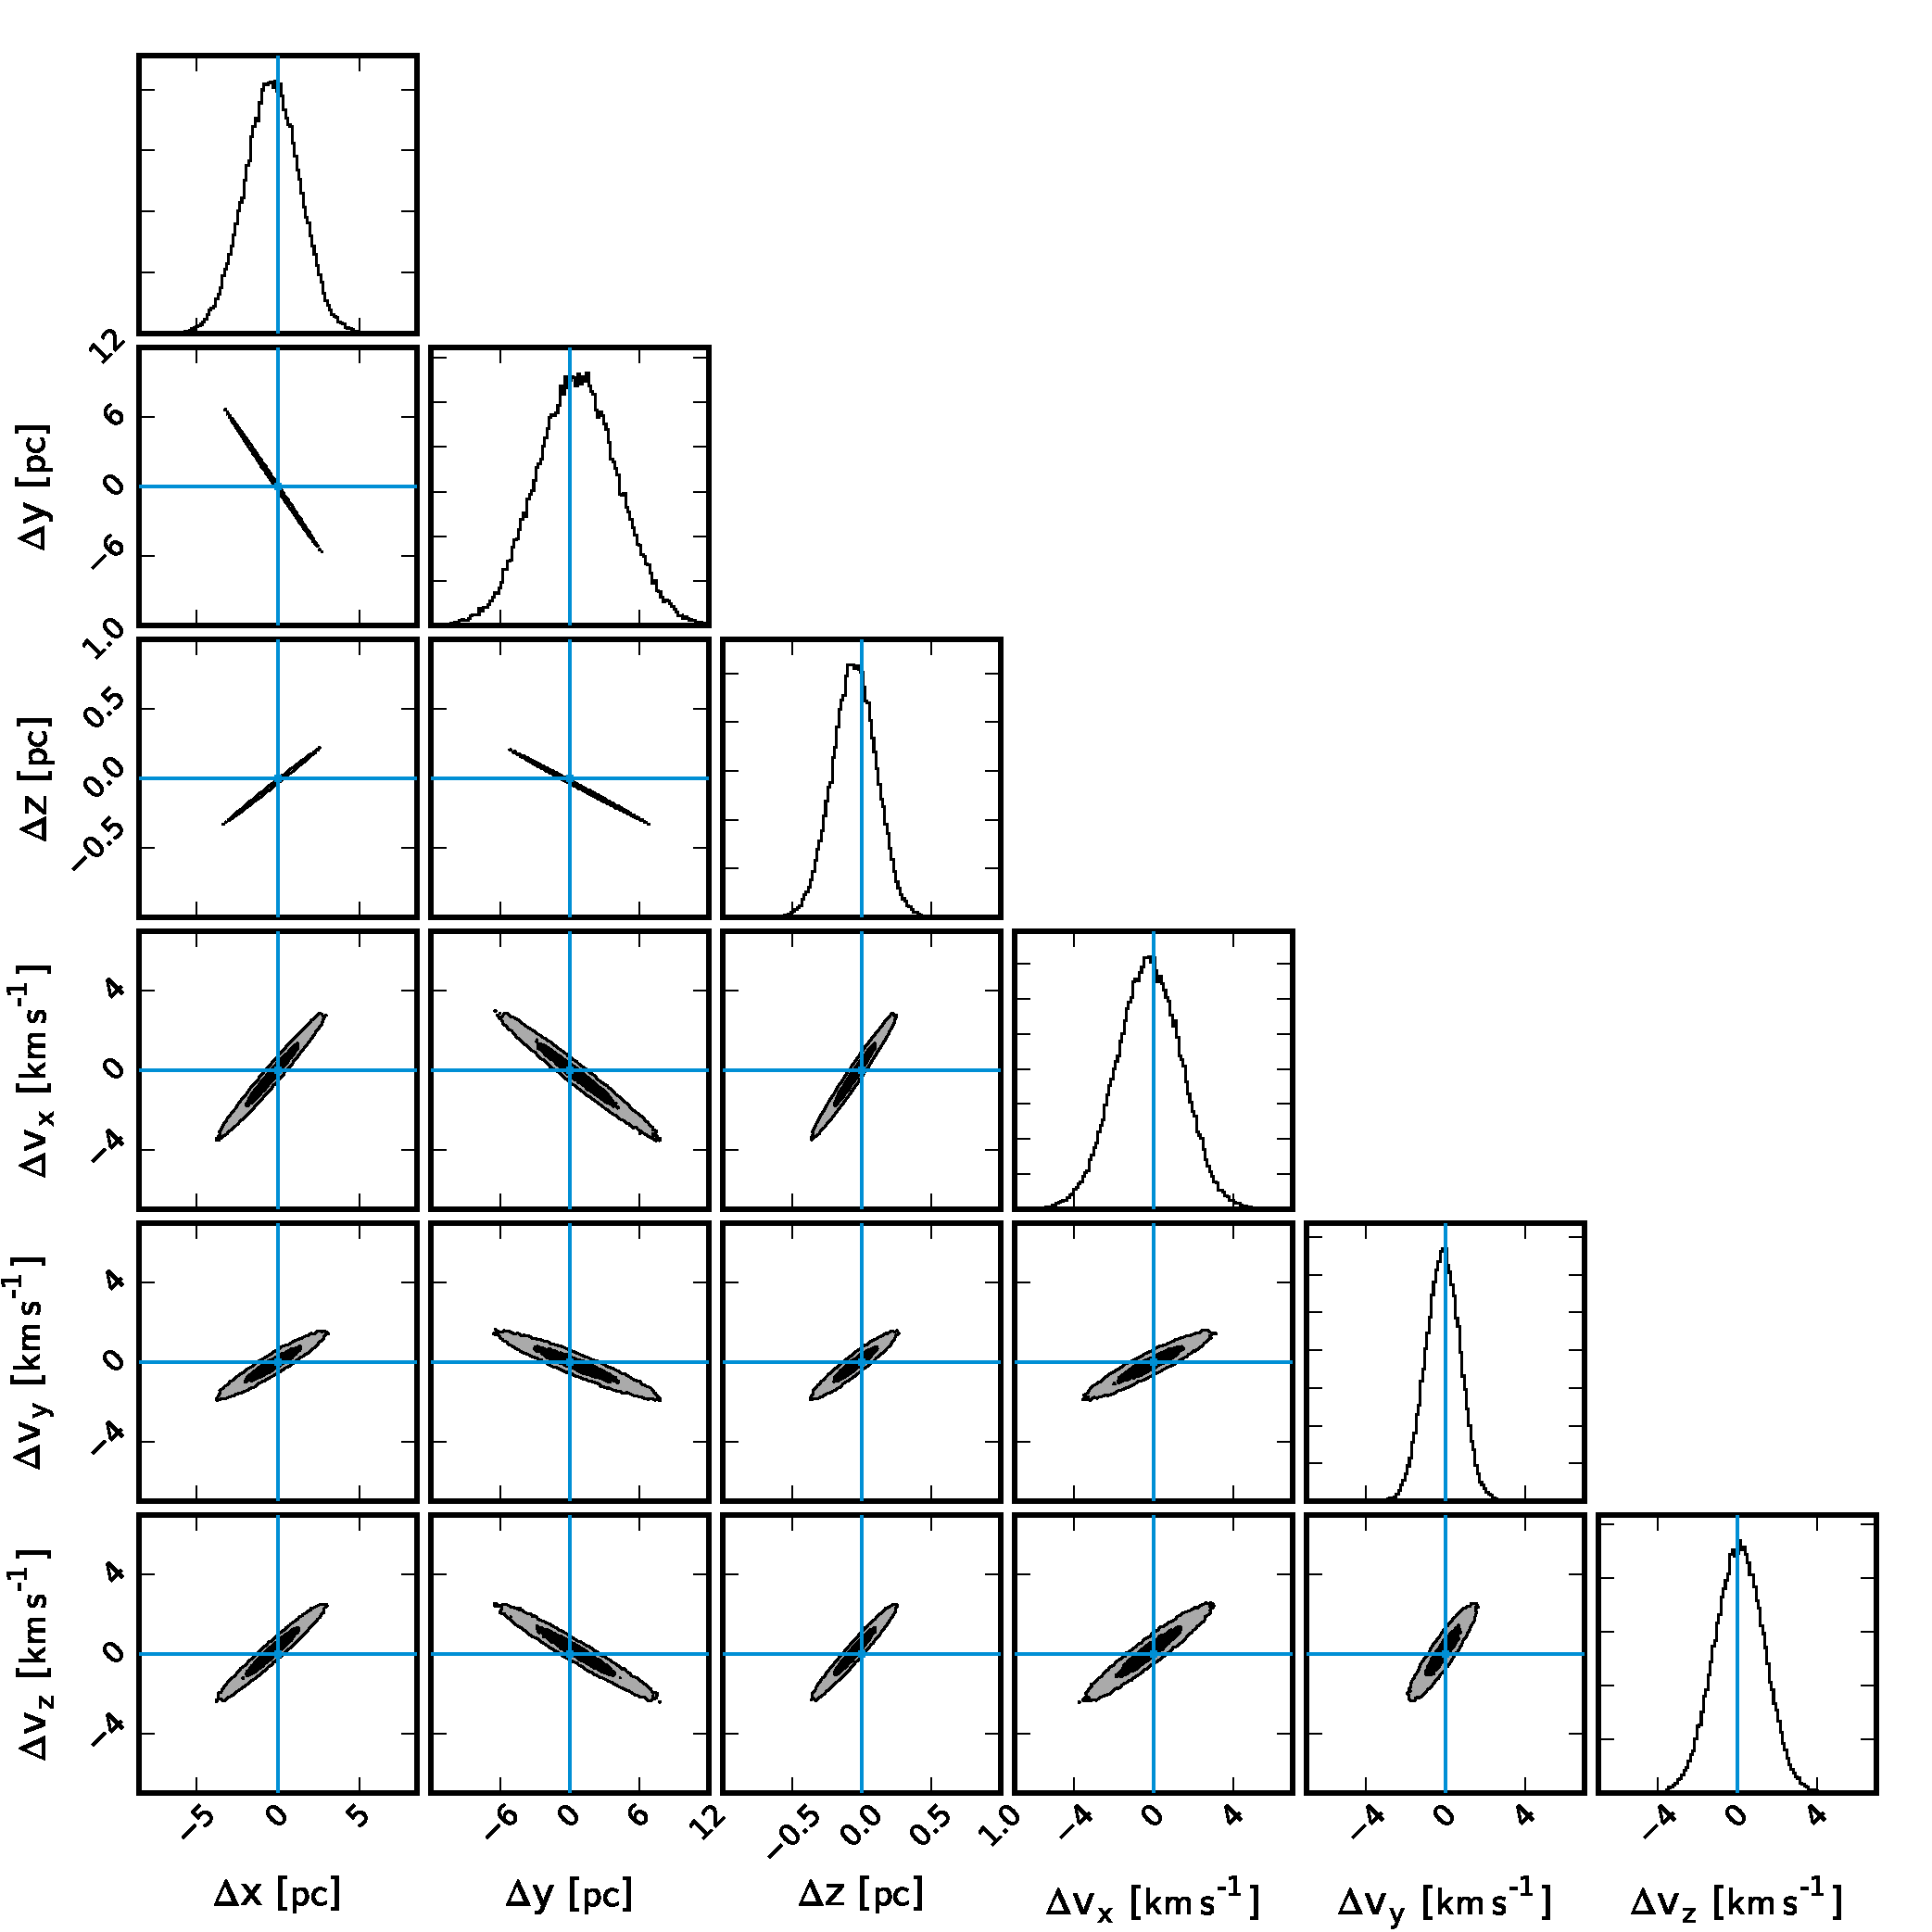
\includegraphics[width=\linewidth]{dx_dv_posterior.pdf}
  \end{center}
  \caption{%
    Differences in posterior samples over Galactocentric phase-space coordinates
    for the two stars \sunanalog\ and \bizarreone.
    \label{fig:dxdv}}
\end{figure}

\figname~\ref{fig:orbit} shows an orbit computed from the median posterior
sample over 6D phase-space coordinates for \sunanalog\ (black line), integrated
in a Milky Way-like gravitational potential (\cite{Gala:2017}). \todo{APW:
explain}
The Sun's orbit in this same Milky Way model is under-plotted for comparison
(grey line); the orbits of the stars in this pair have large scale-heights
relative to the Sun's orbit despite being young.

\begin{figure}[htbp]
  \begin{center}
    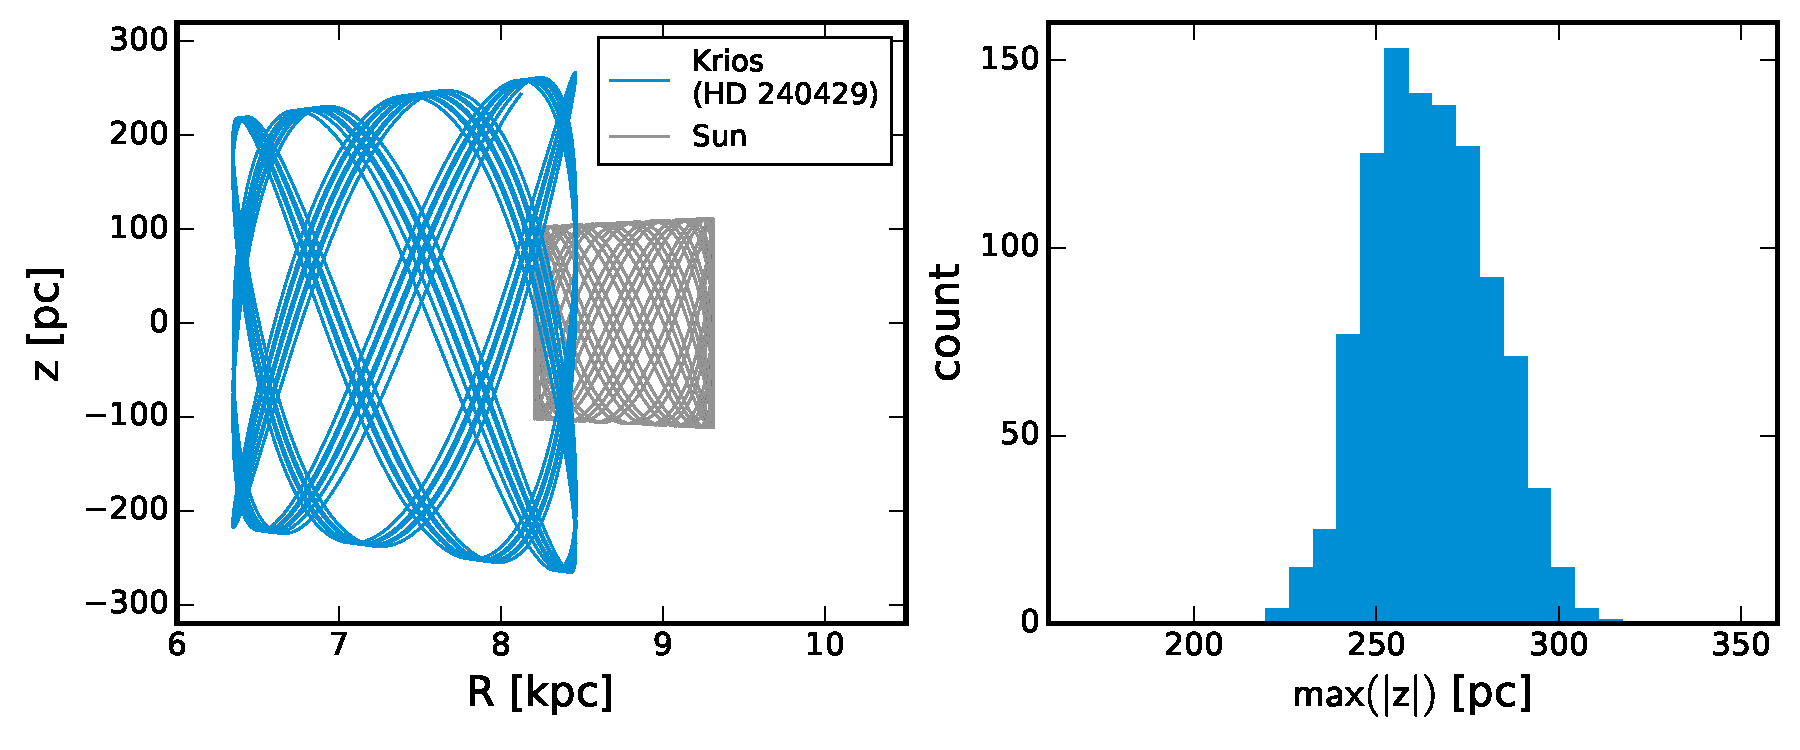
\includegraphics[width=\linewidth]{orbits.pdf}
  \end{center}
  \caption{%
    Galactic orbits computed for \sunanalog\ (black) and the Sun (grey).
    For \sunanalog\, the initial conditions are set to the median posterior
    sample over the inferred 6D phase-space coordinates.
    The orbits are computed by integrating backwards from the present-day
    positions for $2.5~{\rm Gyr}$ with a time-step of $0.5~{\rm Myr}$ using the
    Leapfrog integration scheme implemented in \project{Gala}
    (\citealt{Gala:2017}). \todo{APW: citation...}
\label{fig:orbit}}
\end{figure}



\todo{Figure: posterior distributions of separation and delta V}

Given their proximity in space and kinematics,
it is generally accepted to assume that the two stars were born coeval
perhaps in a wide binary from the same birth cloud.
Thus, we expect the two stars to have identical metallicities and abundance patterns,
\todo{except for thoese elements like Li...}
Surprisingly, one of the stars, \bizarreone\ is significantly more metal
rich than the other by 0.2~dex ($\approx 60\%$; \figname~\ref{fig:abundances}).
What is more puzzling is that the abundances of this star
shows selective depletion in C, N, O, Na, and Mn.

The abundance of \bizarreone\ is peculiar on its own compared to other disk stars with
similar $[\elem{Fe}/\elem{H}]$.
For a star with $[\elem{Fe}/\elem{H}] \approx 0.2$, we generally expect
$[\elem{Na}/\elem{Fe}] > 0$ and $[\elem{Mn}/\elem{Fe}] > -0.1$
(\citealt{Battistini:2015aa,Bensby:2003aa}) making the abundances of \bizarreone\ ever more unlikely.
We stress that none of the other seven binary pairs examined in \citealt{2016ApJS..225...32B}
show discrepancies in abundances between the stars at this level.
In fact, no strong trend is found in pair for most elements
except N and Y.
For Y, the trend for this pair is opposite of the others in Teff.
Specifically, no difference within pair is found for Mn.
(see figure X in that paper; purple is this pair)

\begin{figure}[htpb]
  \centering
  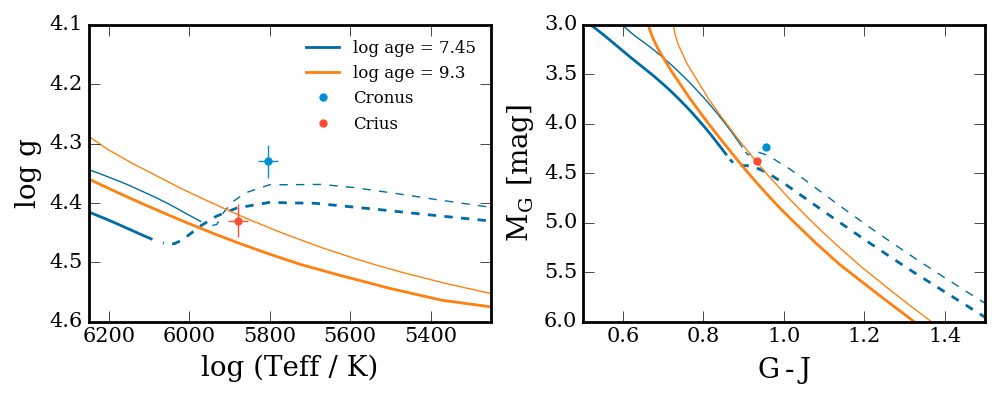
\includegraphics[width=0.95\linewidth]{isochrones.png}
  \caption{Isochrone ages of \sunanalog\ and \bizarreone.
    On the left, we show the two stars on $T_\mathrm{eff}-\log(g)$ plane,
    and on the right, the color-magnitude diagram using \gaia\ $G$ band
    and \tmass\ $J$ band magnitudes.
    In each panel, \project{MIST} isochrones (\citealt{Choi:2016aa}) at $28$~Myr and $2$~Gyr are
    plotted. The thicker and thinner lines are for $\feh = 0.$ and $0.2$,
    corresponding to values of \sunanalog\ and \bizarreone.
  }
  \label{fig:isochrones}
\end{figure}

\begin{figure}[htpb]
  \centering
  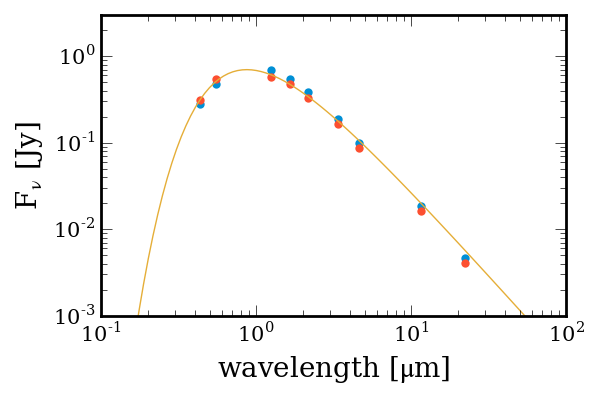
\includegraphics[width=0.8\linewidth]{sed.png}
  \caption{Spectral energy distributions (SEDs) of \sunanalog\ and \bizarreone.
    The yellow line is the SED of a blackbody at $T=5878$ scaled arbitrarily.
  }
  \label{fig:sed}
\end{figure}


The fact that the two stars share a very similar space motion
at a separation of $0.6$~pc strongly argues that the pair is coeval.
We consider other age indicators apart from their phase space coordinates
to assess the ages and coevality of the two stars.
First, given the precise measurements of $\log(g)$, $T_\mathrm{eff}$,
comparing these values to theoretical isochrones may also be indicative of the two stars' ages.
We perform isochrone fitting using the Yale-Yonsei model isocrones (\todo{CITE}).
The input data are $\log(g)$, $T_\mathrm{eff}$, \feh, parallaxes, $B$-band magnitudes, and their errors.
The isochrone ages of \sunanalog\ and \bizarreone\ are
$4.00_{-1.56}^{+1.51}$~Gyr and $4.28_{-1.03}^{+1.11}$~Gyr, respectively,
consistent with them being coeval.

Surface lithium abundance in a sun-like star decreases with its age
due to mixing induced by convection or rotation, which brings the lithium
into the interior ($T>2.5 \times 10^{6}$~K)
where it will be destroyed by proton capture burning.
Thus, surface lithium abundance is an indicator of stellar ages.
The $\elem{Li}$ abundance of $2.25$ for \sunanalog\ implies an age of $\lesssim 1$~Gyr
according to the theoretical models tuned to explain the solar lithium abundance
and rotational profile (\citealt{2005Sci...309.2189C}).
The lithium abundance of \bizarreone\ is still higher by $0.5$~dex
showing the largest difference among all measured elements.
This translates to $\sim 500$~Myr difference in age.
Given the overall higher metal abundances and the peculiar abundance patterns in \bizarreone,
it is unclear, however, whether this higher $\elem{Li}$ abundance
means a younger age or something else.
For example, the presence of $\elem{Li}$-rich red giant stars has been attributed
to the engulfment of substellar companions such as gas giant planets or brown dwarfs
which may replenish $\elem{Li}$ (\citealt{Casey:2016aa}).

In fact, the surface lithium abundance is the only indication that points to younger ages.
If the two stars are indeed only several hundred Myrs old at most,
they are expected to be part of a larger comoving group of stars.
However, as we mention above, there is no evidence in our search of comoving pairs
using \tgas\ that the two stars belong to a larger group of young stars.
Very young stars are often show signs of activity such as
X-ray emission from magnetic activity, emission lines, or infrared excess due to
circumstellar disks.
We have looked for these signs for the pair to find none, and their spectral energy
distribution is consistent with blackbody.
The low $v\sin(i)$ values also argue against very young ages inferred from the
surface lithium abundances.
% TODO: ref for vertical action as age?
Finally, their fiducial orbit in a Milky Way-like potential show that the vertical action
for this pair is larger than the Sun, favoring an older age.
We concluded that the two stars are most likely coeval, $\sim 4$~Gyr old main sequence
stars, and that their unusually high \elem{Li} abundance requires an alternative explanation.

\begin{figure}[htpb]
  \centering
  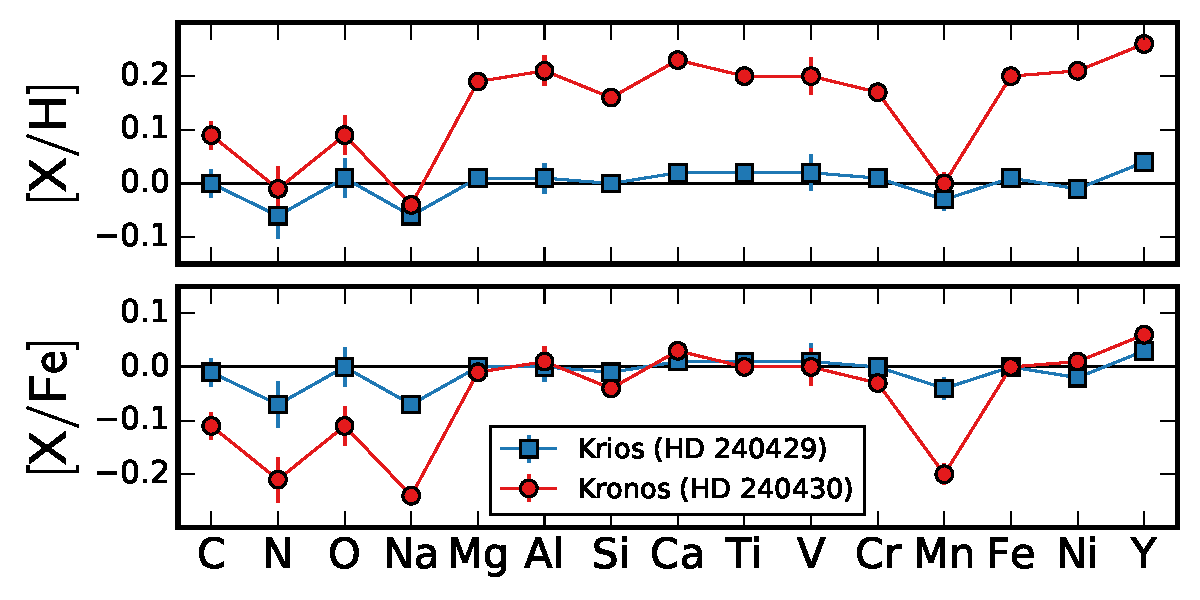
\includegraphics[width=0.9\linewidth]{abundances.pdf}
  \caption{Abundances of the comoving pair, \sunanalog\ and \bizarreone.}
  \label{fig:abundances}
\end{figure}

\begin{figure}[htpb]
  \centering
  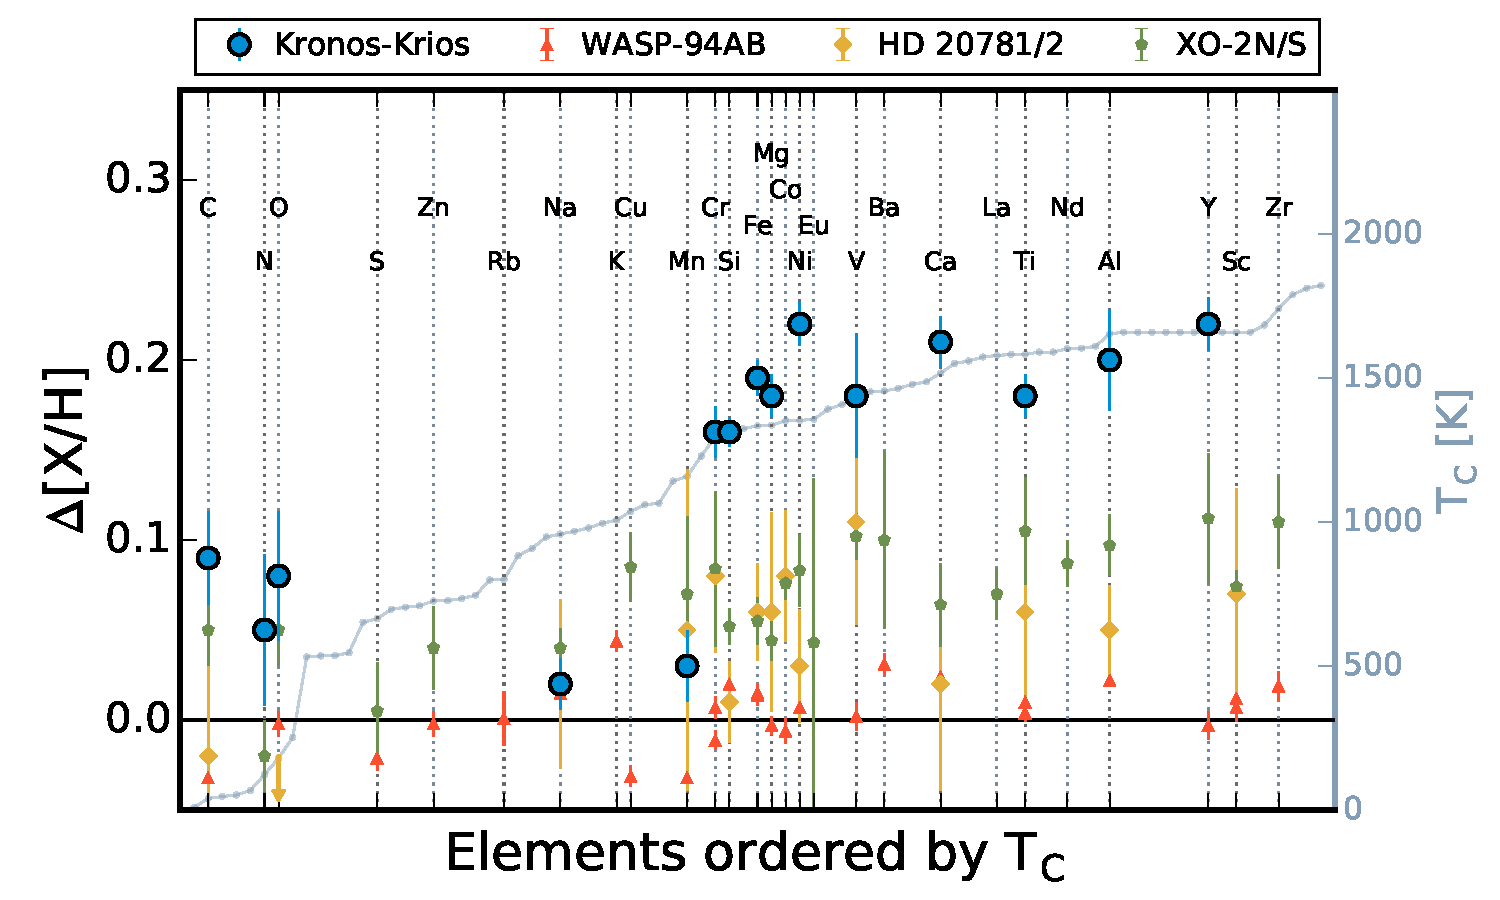
\includegraphics[width=0.95\linewidth]{TcRank_deltaXH_concise.pdf}
  \caption{Abundance of \bizarreone\ ($[\mathrm{Fe}/\mathrm{H}] = 0.20$)
    relative to \sunanalog\ ($[\mathrm{Fe}/\mathrm{H}] = 0.01$)
    as a function of condensation temperature of elements (\citealt{2003ApJ...591.1220L}).
  }
  \label{fig:relabun_tcrank}
\end{figure}

\begin{figure}[htpb]
  \centering
  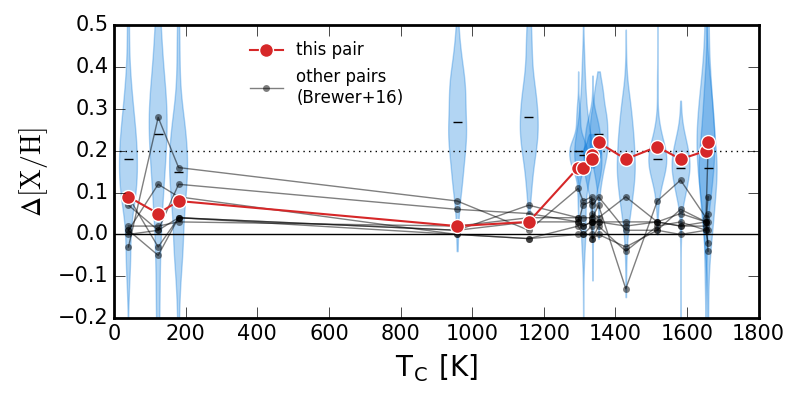
\includegraphics[width=0.9\linewidth]{deltaXH_Tc_violins.png}
  \caption{Difference in abundances of this pair and other binary pairs in
    \citealt{2016ApJS..225...32B}.
    Additionally, we show the distribution of abundance difference
    between stars with similar metallicity difference
    ($\Delta[\elem{Fe}/\elem{H}] \approx 0.2$)
    as violins with medians indicated by black line segments
    by randomly pairing up single stars at two metallicity bins similar to
    the pair of interest.
    The difference is always relative to the lower-$[\elem{Fe}/\elem{H}]$ star.
  }
  \label{fig:deltaXH}
\end{figure}

\section{Discussion}
\label{sec:discussion}

We discuss the possible origins of this pair.
Let us first consider scenarios in which the two stars are not actually born together.

% chance pair
Given that their metallicities and abundance patterns are significantly
different, one may simply conclude that the two stars are not related (coeval)
but they merely happen to be comoving at such small separation ($\approx 0.6$~pc)
by chance.
The two stars are in the Galactic disk, and assuming certain velocity ellipsoid
at the stars' location, one may compute the probability that a star moving at
the mean velocity of the two stars would have a companion within $\Delta v = XX$~km/s.
...

% binary-single and binary-binary exchange
Two stars unrelated at birth may end up in a binary system via binary-single scattering event
that results in an exchange of binary member.
In order to estimate the rate at which any binary-single
event will produce a wide binary system such as \sunanalog\ and \bizarreone,
we may consider the rate at which this wide binary will scatter with a field star to
result in an exchange reaction.
The cross-section of exchange scattering for a binary with semi-major axis $a$ is
\begin{eqnarray}
  \sigma_\mathrm{ex} = \frac{640}{81} \pi a^{2} \frac{1}{v^6}
\end{eqnarray}
where $v$ is the incoming velocity $v_i$ in units of critical velocity $v_c$ defined as
\begin{eqnarray}
  v_c^2 = G \frac{m_1 m_2 (m_1 + m_2 + m_3)}{m_3 (m_1 + m_2)} \frac{1}{a}
\end{eqnarray}
when $v \gg 1$ using the impulse approximation (\citealt{Hut:1983aa,Hut:1983ab}),
which is appropriate for wide binaries scattering with field (disk) stars.
If we assume that field stars are made of solar mass stars
with constant number density $n=1$~pc$^{-3}$, and the incoming velocity of field stars
is $10$~km\,s$^{-1}$, a lower limit to the velocity dispersions of disk
stars in any direction, the rate of exchange scattering is
\begin{eqnarray}
  n \sigma_\mathrm{ex} v_i = 6.82\times 10^{-8}\,\mathrm{Gyr}^{-1}
  \frac{n}{\mathrm{pc}^3} \frac{\mathrm{pc}}{a} \left(\frac{10~\mathrm{km}\,\mathrm{s}^{-1}}{v_i}\right)^5
\end{eqnarray}
low enough to be negligible.
Because the exchange scattering cross section steeply depends on the incoming velocity
relative to the critical velocity (of the order of orbital velocity of the binary),
the rate of exchange scattering with a star within the same star forming region
may be much larger.
However, even in such scenario, the age difference of $\sim 500$~Myr is too large
for two stars of the same star forming region.

In regions where binarity fraction is high, binary-binary scattering may be more important
than binary-single scattering (\todo{CITE})


%Two factors that make this even more unlikely are that both stars are very young given their large Li,
%and that if the pair is a result of scattering, one expect to end up with typical stars of the field,
%not HD30 with anomalous abundance patterns.


None of the above scenarios is satisfactory as they offer no
insight on the peculiarity of the abundances of \bizarreone\
(see \sectionname~{\ref{sec:data}}).
In case that the pair formed from a exchange scattering event,
we would expect the pair to be composed of typical field stars.
The unlikeliness of the above possibilities naturally leads us to
consider the alternative.
What can selectively enrich refractory (high $T_C$) elements
in one of the two stars that are born together?

% inhomogeneity in star formation
It may be that the two stars are born at the same time from the same cloud, but
there is inhomogeneity within the cloud.
However, there is already ample amount of evidence against such scenario.
First, none of the other seven similar wide binaries examined in \citealt{2016ApJS..225...32B}
show the same level differences in abundances although there is generally
a larger spread in $\elem{C}$, $\elem{N}$ and $\elem{O}$, and some pairs show
a large as $\approx 0.15$~dex difference in particular elements.
The median and maximum \feh\ difference between component stars in the other seven pairs
is $0.02$~dex and $0.09$~dex, respectively.
This is consistent with the findings of \citealt{Desidera:2004aa}, who examined 23 wide binaries
of late F to K dwarfs, and found most pairs show difference in \feh\ less than $0.02$~dex
and none larger than $0.07$~dex.

% rocky planets (or the like) engulfment
Yet another possibility that may change a star's surface abundance after formation
is accretion of its planets or asteroids.
Instabilities may develop in a multi-planet system due to chaotic
nature of many body system, which may lead to planet engulfment by the host star.

One informative proxy that may reveal the composition of the hypothetical material
that was accreted to the stars is the condensation temperature.

Present the relative abundance figure here

One can carry out simple toy calculations of expected $\Delta\elemH{X}$
in a Sun-like star's atmosphere when adding material of e.g., bulk Earth composition
under these assumptions:
\begin{itemize}
  \item The material added is instantly and completely mixed.
  \item The atmospheric composition that we measure is identical throughout
    the star's radiative and convective zone.
\end{itemize}
We take the solar abundances $\elemH{X}$ of \citealt{Asplund:2009aa}
which can be converted to mass fraction in each element $X$ as in
\begin{equation}
  f_{X,\mathrm{photo}} = \frac{10^{\elemH{X}} m_X}{\Sigma_X 10^{\elemH{X}} m_X}
\end{equation}
where $m_X$ is the mass of each element in e.g., atomic mass unit.
One can check that the \citealt{Asplund:2009aa} abundances
are consistent with mass fraction in \elem{H}, \elem{He} and metals
$X,\,Y,\,Z=0.757,\,0.249,\,0.0134$ as stated in that work.
Assuming a fraction of the star's convective zone in mass $f_\mathrm{CZ}$,
and that the added material has a total mass $M_\mathrm{add}$ and mass fraction in each
element $f_{X,\mathrm{add}}$,
the abundance difference is
\begin{equation}
  \Delta\elemH{X} = \log_{10} \frac{f_{X,\mathrm{photo}}\,f_\mathrm{CZ}\,M_\mathrm{star} + f_{X,\mathrm{add}}\,M_\mathrm{add}}
    {f_{X,\mathrm{photo}}\,f_\mathrm{CZ}\,M_\mathrm{star}}
\end{equation}
We take the composition of bulk Earth from a chondritic model of the Earth
(\citealt{mcdonough2001composition}) and CI chondrite from \citealt{2009LanB...4B...44L}.

Figure~\ref{fig:toycalc} shows the expected change of surface abundances in a
Sun-like star after $20~\mearth$ of material with composition of bulk Earth or
CI chondrite is added.
The CI chondrites are believed to have the closest in composition to the solar nebular.
Their composition closely matches that of the solar atmosphere except
Li, highly volatile ($\Tcondens < 250$~K) elements, and the noble gases.
Other groups of chondrites show differing level of variations from CI chondrites.
It has been long known that compared to CI or other carbonaceous chondrites,
the composition of the Earth shows a volatilaity trend that moderately volatile
elements (including Mn and Na) and volatile elements are incearsingly more
depleted with decreasing condensation temperature (\citealt{mcdonough2001composition}).
This trend is presumed to be closely related to the formation of terrestrial planets.
Given the simplistic assumptions laid out above, and the uncertainties
in our current knowledge of the compositions of terrestrial planets including bulk Earth,
the match between our toy calculation and the observed abundance difference
between \bizarreone\ and \sunanalog\ is remarkable.

% some discussion of individual elements

The element \elem{Li} is worth a special attention in the context of accretion scenario.
Because Li is present in either carbonaceous chondrites or the bulk Earth with
a concentration of $1-1.5$~ppm in mass (\citealt{mcdonough2001composition,}),
but is depleted over time on the surface of a Sun-like star, accretion of
either at later time will significantly replenish the lithium on the star's
surface.
For the present-day Sun, the accretion of $20~\mearth$ of bulk Earth-like
material results in $\Delta\elemH{Li} \approx 1.6$~dex.
Incidentally, the star under examination, \bizarreone, has an age (informed by
stellar parameters) very close to the Sun ().
Thus, as long as we believe the Sun's present-day surface Li abundance
to be ordinary, this predicts that the \bizarreone\ should have $1.6$~dex enhancement
in its Li.
This is in fact exactly what we find: the Li abundance of \bizarreone\ is
$A(\elem{Li}) = 2.75$ (Table~\ref{tab:kk}, \todo{CITE JM?})
approximately $1.6$~dex higher than the solar value of $1.1$~dex.
Furthermore, this implies that the accretion event should have happened
very recently from a time ago that is shorter than the \elem{Li} depletion time.

It is further worth pointing out that measuring the \elem{Li} abundance
with some of the refractory elements such as $\elem{Fe}$
provides a way to estimate the time of the event.
If the observed \elem{Li} abundance is less than what is inferred from
abundance differences of other elements, and
we have a model of \elem{Li} depletion, the time of \elem{Li} enhancement
may be calculated.

What about \sunanalog?
\sunanalog\ is also enhanced in \elem{Li} considering its age of $4.00_{-1.56}^{+1.51}$~Gyr
than the nominal \elem{Li} depletion predics by $\approx 1$~dex.
This enhancement puts an upper limit on the accreted mass to be \todo{$\approx 4$~\mearth}
assuming \elem{Li} concentration of $1.1$~ppm (\citealt{mcdonough2001composition}).
Unlike \bizarreone, we cannot know the pre-accretion abundances of \sunanalog.
However, we note that the span of abundance difference between highly volatile elements
(C, N, O, Na) and refractory elements such as \elem{Fe} expected from accreting
\todo{$\approx 4$~\mearth} to the Sun is $\approx 0.05$~dex.
This is comparable to the abundance difference between N, Na and Fe in \sunanalog.
It is also interesting that \sunanalog\ also shows a deficit in the same
volatile and moderately volatile elements (C, N, O, Na, and Mn) relative to Fe
just as in \bizarreone.
Thus, we conclude that \sunanalog\ is also likely to have had a similar
accretion event, but the amount of accretion was much smaller than \bizarreone.

We stress that
% - these calculations are carried out with very simple and unverified assumptions
% - uncertainties exist on the bulk Earth







\begin{figure}[htpb]
  \centering
  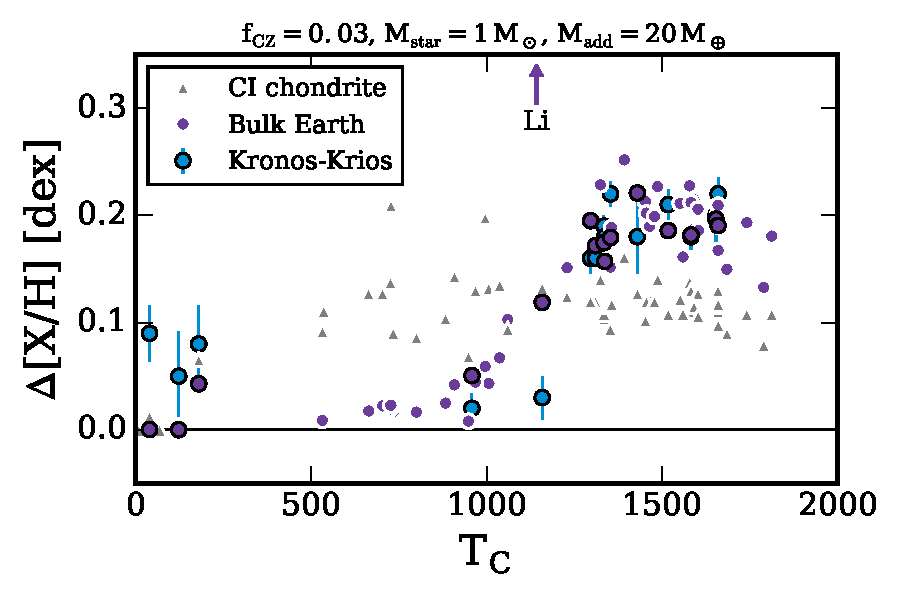
\includegraphics[width=0.8\linewidth]{toycalc.pdf}
  \caption{Solar surface abundance change expected from adding $20~\mearth$ of
    material with bulk Earth or CI chondrite composition.
    The assumed mass fraction in the convective zone is $0.03$.
    For bulk earth composition, which is a closer match to the abundance difference
    seen in \bizarreone\ and \sunanalog, we indicate measured elements with black boundary
    lines around symbols.
  }
  \label{fig:toycalc}
\end{figure}




\input{otherstudies.tex}

We summarize the few wide separation common proper motion pairs that have been
studied in detailed chemical abundance so far.
These systems are HD~20782/HD~20781, HD~80606/HD~80607, XO-2N/XO-2S, HAT-P-1,
WASP-94A/WASP94-B, and HD~133131A/HD~133131B.
Main properties of the systems relevant to the present discussion are
summarized in \tablename~\ref{tab:otherstudies}.
Their reported abundance differences $\Delta\elemH{X}$ where the difference is
always taken as $\mathrm{higher}~\feh - \mathrm{lower}~\feh$ are plotted in
\figname~\ref{fig:relabun_tcrank} as a function of \Tcondens-rank for
comparison with this pair.

{\bf HD~20782/HD~20782:} 
\citealt{Mack:2014aa} studied HD~20782/20781, two common proper motion G dwarf stars (G2/G9.5)
with a projected separation of $\sim9000$~AU (corresponding to 4.2~arcmin sky separation).
Both stars in this system host close-in giant planets.
HD~20782 hosts a Jupiter-mass planet on a very eccentric ($e\approx 0.97$) orbit with a
pericenter distance of 1.4~AU while HD~20781 hosts two Neptune-mass planets within 0.3~AU
with moderately high eccentricity ($e\sim0.1-0.3$).
They found that the abundances of 15 elements between the two stars are consistent with each other.
However, they argued that there is a moderately significant ($\sim 2\sigma$)
positive slope of $\approx 10^{-5}$~dex\,K$^{-1}$ in abundance of each star
{\it individually} with increasing \Tcondens\ for $\Tcondens>900$~K elements
(namely, Na, Mn, Cr, Si, Fe, Mg, Co, Ni, V, Ca, Ti, Al, Sc leaving out C and O
of their measurements).
They interpreted that this slope may be evidence for accretion of $10-20$~\mearth\ of 
H-depleted rocky material that were pushed in during giant planet migration.

{\bf WASP-94A/WASP-94B:} 
\citealt{Teske:2016aa} studied WASP-94A/WASP-94B, a pair of F8 and F9 stars
with super-solar metallicity ($\feh\approx 0.3$ for both stars). Both stars
host a hot Jupiter.
The planet hosted by WASP-94A is transiting with a misaligned, probably
retrograde circular ($e<0.13$) orbit, while that hosted by WASP-94B is a little
more massive by $\sim 0.15$~\mjupiter\ and closer in, aligned with the host
star.
With a claimed median uncertainty of $0.006$~dex among all elements, they
detected a depletion of volatile and moderately volatile ($\Tcondens < 1200$~K)
elements at $0.02$~dex level and an enhancement in refractory ($\Tcondens >
1200$~K) elements at $0.01$~dex level in WASP-94A relative to WASP-94B.
Excluding K, which is based on one strong line and largely affected by non-LTE
effect, their analysis shows a statistically significant non-zero slope between
$\Delta\elemH{X}$ and $\Tcondens$\footnote{Note that the condensation
  temperature $\Tcondens$ used is for solar (system? atmosphere?) composition
  gas, which can differ from that of higher metallicity gas.}.
They considered multiple possibilities related to the formation and evolution
of planetary systems around each star as well as causes unrelated to planets
such as dust cleansing during the fully convective phase or different rotation
and granulation between the stars, but did not favor any particular one.

{\bf HD~80606/HD~80607:}
The pair of G5 stars HD 80606/HD 80607 has been independently studied by
\citealt{Saffe:2015aa} and \citealt{Mack:2016aa} using the same KECK HIRES
spectra. HD 80606 hosts a giant planet with mass of $4~\mjupiter$ at $0.5$~AU
on a very eccentric ($e\approx0.95$) orbit while HD 80607 has no detected
planets.
Both stars are super solar with $\feh=0.35$.


{\bf HAT-P-1:}
HAT-P-1 is a pair of G0 stars separated 11\farcs apart in sky
with $\feh\approx0.15$.
The secondary star in the system is known to host one transiting giant planet
while no planet has been discovered around the primary star.
\citealt{Liu:2014aa} found that the two stars are identical in their atmospheric composition:
\feh\ is $0.146 \pm 0.014$ and $0.155 \pm 0.007$ for the primary and secondary respectively,
and $\Delta\elem{X}/{Fe}$ is consistent with zero for 23 elements measured
with the mean error being $0.013$~dex.
Based on this analysis, they concluded that the presence of close-in giant planet
does not necessarily lead to stellar atmospheric pollution of the host star.

{\bf XO-2N/XO-2S:}
The double star system XO-2 has received much attention due to
possibly the most robust and significant difference between the component stars
among those so far studied.
XO-2 is a pair of G9 stars with super-solar metallicity ($\feh \gtrsim 0.35$),
each hosting planet(s).
XO-2N hosts on giant planet while XO-2S is known to host two giant planets with
masses $0.26 \mjupiter$ and $1.37 \mjupiter$ on moderately eccentric ($\approx
0.15$) orbits at $<0.5$~AU.

The system was first analyzed by \citealt{Teske:2013aa}, who examined and found
essentially no significant difference in Fe, Ni, C, and O between the two
stars.
However, re-analysis of the system using the same data in
\citealt{Teske:2015aa} found that the trend of $\Delta\elemH{X}$ with
\Tcondens\ varies significantly depending on the stellar parameters chosen in
their analysis. Both analyses were based on spectra
using Subaru High Dispersion Spectrograph at spectral resolution $R=60000$
covering $4450-5660~\AA$ and $5860-7100~\AA$ with S/N of $170-230$
(\citealt{Teske:2013aa}).

Independently, \citealt{Ramirez:2015aa} used Keck HIRES spectra ($R=67000$,
$4080-8300~\AA$) of the component stars with S/N of $350$ (in $5000-7500~\AA$)
to perform a differential abundance analysis.
They find that all 23 elements including Fe is enhanced in XO-2N
compared to XO-2S, and that the difference $\Delta\elemH{X}$ shows
a significant correlation with \Tcondens.
At low \Tcondens, volatile elements differ by $0.015$~dex
while the range of difference spans upto $0.1$~dex at $\Tcondens>1600$~K.
There are inconsistencies in the determination of stellar parameters
(\teff\ and \logg) between spectroscopic (based on Fe I/II lines)
and photometric analysis,
but the existence of correlation between $\Delta\elem{H}$ and
\Tcondens\ seems robust.

\citealt{Ramirez:2015aa} argued that the {\it depletion} of
volatile elements in XO-2S relative to XO-2N is plausibly
due to {\it more} gas giant planets around XO-2S,
following a similar interpretation of \citealt{Melendez:2009aa}
on the trend between solar twins and the Sun.
In this scenario, forming planets in the protoplanetary disk
are supposed to ``lock'' heavier elements to the core of gas giant
planets as well as some volatile elements in their envelopes.
Then, the host star will somehow accrete {\it gas} depleted in
metals compared to their protostellar condition.
By tuning the metal content ($Z/X$) of gas giant planets
and when the accretion of gas occurs in terms of how much mass
is in the convective envelop then, they can match
the mass difference of gas giant planets around each star,
which is at least $1~\mjupiter$.
For the positive correlation of $\Delta\elemH{X}$ with \Tcondens,
\citealt{Ramirez:2015aa} estimated that $20~\mearth$
of equal-part mixture of Earth and CM chondrite-like material
can explain the trend either as
refractory {\it depletion} in XO-2S due to {\it more} rocky planets
around XO-2S, or refractory enhancement in XO-2N by late time accretion
in which case the complete opposite would be true.

Finally, \citealt{Biazzo:2015aa} 






% Useful follow up efforts
We discuss the follow up efforts that would be useful to further
illuminate the peculiar abundance difference between the pair.



\section{Summary}
\label{sec:summary}

We have reported and discussed the discovery of a comoving pair of bright solar-type stars
HD~240430 and HD~240429 (G0 and G2)
with very different metallicity ($\Delta\feh \approx 0.2$~dex),
and a condensation temperature-dependent abundance difference.

% Concluding remarks


\begin{figure}[htpb]
  \centering
  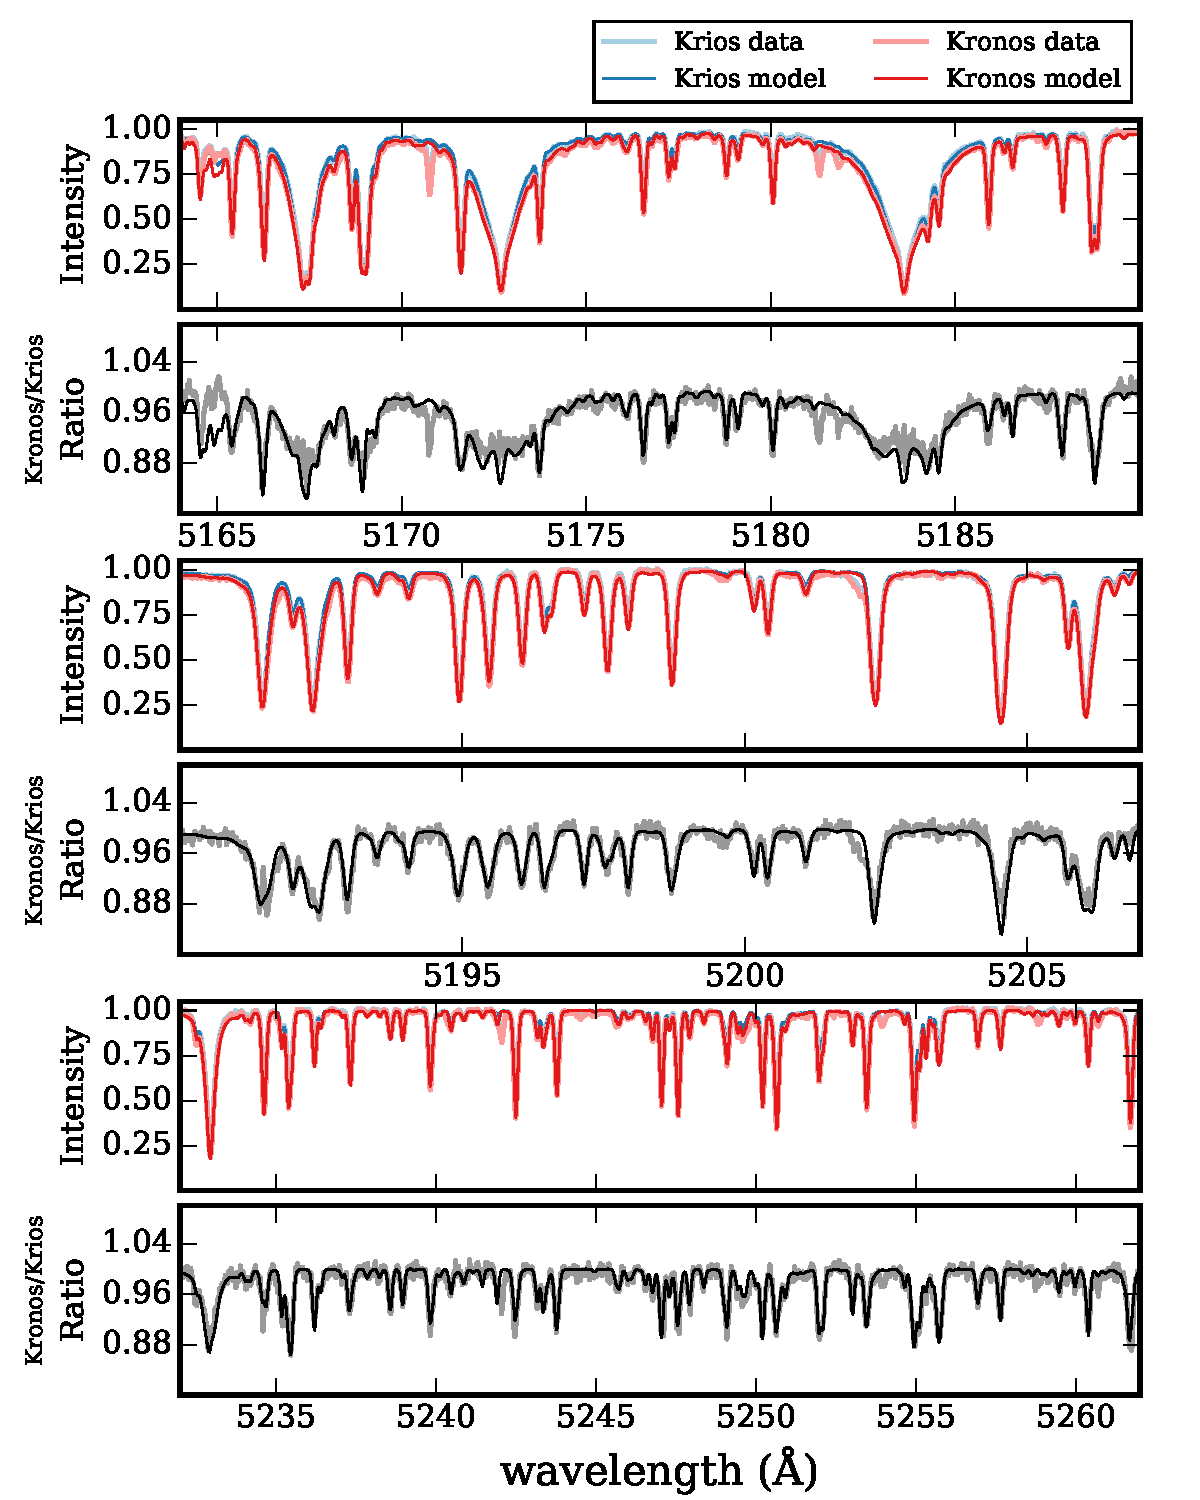
\includegraphics[width=0.95\linewidth]{spec1.pdf}
  \caption{Selective segments of the spectra of \sunanalog\ and \bizarreone.
    For each row, the continuum-normalized data and model are plotted in the upper panel,
    and the ratio (\bizarreone/\sunanalog) of data (gray) and model (black)
    are plotted in the lower panel.
  }
  \label{fig:spec1}
\end{figure}

\begin{figure}[htpb]
  \centering
  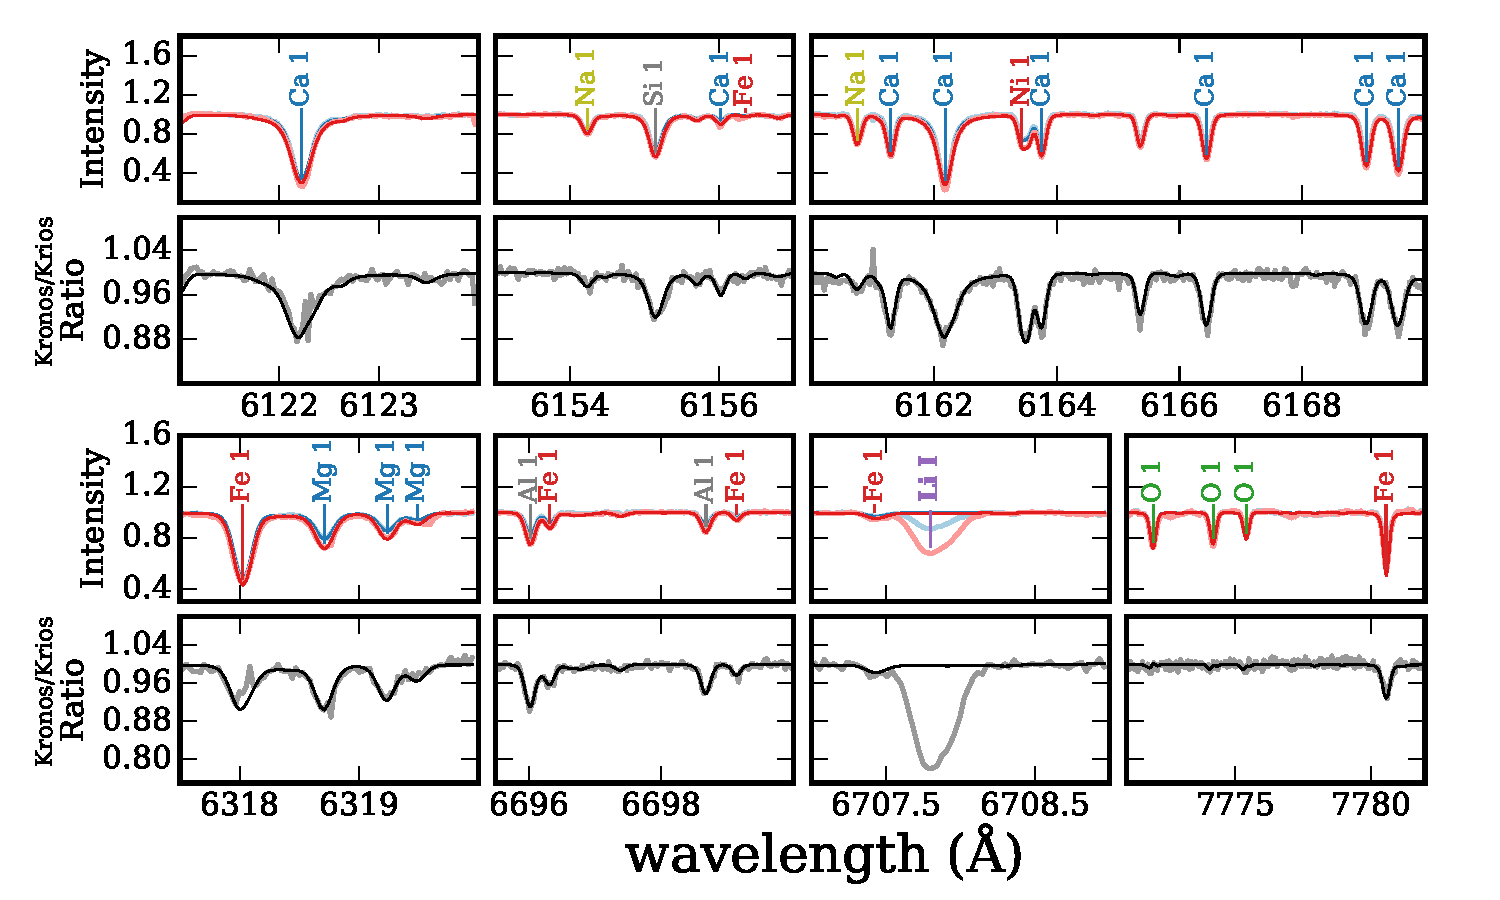
\includegraphics[width=0.95\linewidth]{spec2.pdf}
  \caption{Same as \figname~\ref{fig:spec1} but for smaller portions of spectra that are
    not dominated by \elem{Fe}. We mark elements that give rise to strong lines.
    The feature in the third column of the second row is a strong \elem{Li} line that was
    not modeled by \citealt{2016ApJS..225...32B}. This line was studied in a separate study
    \todo{CITE}.
  }
  \label{fig:spec2}
\end{figure}

\bibliography{ref}



\end{document}
